%%%%%%%%%%%%%%%%%%%%%%%%%%%%%%%%%%%%%%%%%
% Data Collections Summary
% LaTeX Template
% Version 2.1 (1/10/15)
%
% This template has been downloaded from:
% http://www.LaTeXTemplates.com
%
% Original author:
% Mathias Legrand (legrand.mathias@gmail.com) 
% With extensive modifications by:
% Vel (vel@latextemplates.com)
%
% License:
% CC BY-NC-SA 3.0 (http://creativecommons.org/licenses/by-nc-sa/3.0/)
%
%%%%%%%%%%%%%%%%%%%%%%%%%%%%%%%%%%%%%%%%%

%----------------------------------------------------------------------------------------
%	PACKAGES AND OTHER DOCUMENT CONFIGURATIONS
%----------------------------------------------------------------------------------------

\documentclass[obeyspaces, spaces, fleqn,10pt]{SelfArx} % Document font size and equations flushed left

\usepackage[english]{babel} % Specify a different language here - english by default

\usepackage{lipsum} % Required to insert dummy text. To be removed otherwise

\PassOptionsToPackage{obeyspaces, spaces}{url}
\usepackage[obeyspaces, spaces]{url}
\usepackage{minted}
\def\UrlBreaks{\do\/\do-}

%----------------------------------------------------------------------------------------
%	COLUMNS
%----------------------------------------------------------------------------------------

\setlength{\columnsep}{0.55cm} % Distance between the two columns of text
\setlength{\fboxrule}{0.75pt} % Width of the border around the abstract

%----------------------------------------------------------------------------------------
%	COLORS
%----------------------------------------------------------------------------------------

\definecolor{color1}{RGB}{0,0,0} % Color of the article title and sections
\definecolor{color2}{RGB}{53 88,118} % Color of the boxes behind the abstract and headings

%----------------------------------------------------------------------------------------
%	HYPERLINKS
%----------------------------------------------------------------------------------------

\usepackage{hyperref} % Required for hyperlinks
\hypersetup{hidelinks,colorlinks,breaklinks=true,urlcolor=color2,citecolor=color1,linkcolor=color1,bookmarksopen=false,pdftitle={Title},pdfauthor={Author}}

%----------------------------------------------------------------------------------------
%	ARTICLE INFORMATION
%----------------------------------------------------------------------------------------

\Archive{May 12, 2019} % Additional notes (e.g. copyright, DOI, review/research article)
\JournalInfo{Data Science 2: CS109B} % Journal information

\PaperTitle{Algorithmic Biases in Facial Recognition} % Article title

\Authors{Whitney Jablonski, Paul Jureidini, Samata Kurhekar, Shourya Veeraganti} % Authors
%\affiliation{\textsuperscript{1}\textit{Department of Biology, University of Examples, London, United Kingdom}} % Author affiliation
%\affiliation{\textsuperscript{2}\textit{Department of Chemistry, University of Examples, London, United Kingdom}} % Author affiliation
%\affiliation{*\textbf{Corresponding author}: john@smith.com} % Corresponding author

\Keywords{} % Keywords - if you don't want any simply remove all the text between the curly brackets
%\newcommand{\keywordname}{Keywords} % Defines the keywords heading name

%----------------------------------------------------------------------------------------
%	ABSTRACT
%----------------------------------------------------------------------------------------

%\Abstract{}

%----------------------------------------------------------------------------------------

\begin{document}

\flushbottom % Makes all text pages the same height

\maketitle % Print the title and abstract box

\tableofcontents % Print the contents section

\thispagestyle{empty} % Removes page numbering from the first page

%----------------------------------------------------------------------------------------
%	ARTICLE CONTENTS
%----------------------------------------------------------------------------------------

%\section*{Summary} % The \section*{} command stops section numbering

%\addcontentsline{toc}{section}{Summary} % Adds this section to the table of contents

%\lipsum[1-3] % Dummy text
% and some mathematics $\cos\pi=-1$ and $\alpha$ in the text\footnote{And some mathematics $\cos\pi=-1$ and $\alpha$ in the text.}.

%------------------------------------------------

\section{Introduction}

Facial analysis and facial recognition are technologies fueled by artificial intelligence that are becoming more entrenched in our every day lives even in a broad range of areas. Applications range from smartphone cameras (e.g., auto-focusing), law enforcement (e.g., border security, risk assessment for recidivism), and advertisement targeting (e.g., from profile pictures).\cite{Couch:2017,Lohr:2018,Kim:2018} The crux of the issue lies in the insufficiently diverse training data sets that introduce bias into machine learning algorithms used in all of the applications listed. Popular, publicly available, and easily accessible data sets such as Labeled Faces in the Wild (LFW) are used by software companies (e.g., Google) for benchmarking their facial recognition machine learning algorithms.\cite{LFWTech,Lohr:2018} In 2015, Google's facial recognition app mistakenly identified black people as gorillas which kicked off a conversation about algorithmic bias and its potential implications for humans.\cite{dough2015,Lohr:2018} Algorithmic bias like that which caused the misidentification of black people can be introduced during training when using data sets such as LFW which Wang et. al. estimated to be nearly 85\% white.\cite{wang:2018}  The resulting model will inherently have more error in identifying underrepresented races, and therefore the algorithm will more accurately predict features of better represented races. 

In this work, we evaluate racial algorithmic bias from the standpoint of gender classification using several publicly available data sets. First, we discuss the selection process for the data set and features of the data, the models used herein, and our choice for using gender classification as a benchmark. Then we detail our approach for image pre-processing, data ingestion to the mode, the model architecture, and augmentation of images for model improvement. Finally, we present a comparison of the performance for gender classification with respect to race for each of the methods outlined. Our overarching goal is to reduce algorithmic bias by training a convolutional neural net (CNN) for gender classification using a more diverse training data set, and then test it against an existing non-diverse training data set (e.g., LFW).

\subsection{Image Data Selection}
A summary of four publicly available facial image databases that we evaluated for this study is given in Table \ref{tab:tab1}. For our purposes, we sought a data set with explicit labels for race and gender. The VGGFace2 data set is the most comprehensive with over 3.3 million faces and more than 8600 identities at different ages.\cite{Cao18} Unfortunately, VGGFace2 is not explicitly labeled for race, and therefore we opted to use the UTKFace data set which was conveniently labeled for both gender and race with a relatively good sample size of 23,000 images.\cite{utkface} We evaluated LFW and a data set created by a group in China called 'Racial Faces in the Wild' with race labels, but neither data set suited our needs for gender labels.\cite{LFWTech,wang:2018} 

\begin{table}[hbt]
\caption{Summary of facial image databases.}
\centering
\begin{tabular}{lclc}
\toprule
%\multicolumn{2}{c}{Name} \\
%\cmidrule(r){1-2}
Name & \# Faces (thousands) & Labels & Ref \\
\midrule
VGGFace2 & ~3,300 & a,g,i & \cite{Cao18} \\
LFW & 13 & i & \cite{LFWTech} \\
RFW & 665 & r,i & \cite{wang:2018} \\
UTKFace & 23 & a,g,r & \cite{utkface} \\
\bottomrule
\multicolumn{4}{l}{age (a), gender (g), race (r), identity (i)} \\
\end{tabular}
\label{tab:tab1}
\end{table}

The UTKFace data was developed by researchers at the University of Tennessee Knoxville (UTK) who were developing a conditional adversarial autoencoder for age progression/regression and sought a racially and age-balanced data set.\cite{utkface} As a result, there is a wide range of ages of the people represented in the images. UTKFace contains images that range in age from 1 to 116 with a mean age of 33. Four races and one aggregated category are represented: white, black, asian, indian, and other (hispanic, latino, middle eastern). A comparison of the distribution for age and race with respect to gender is shown in Figure \ref{fig:fig2}. Male and female are represented fairly equally among the races with slightly more male images in the white and indian categories and slightly more female images in the asian and other categories. We are not explicitly dealing with age for our analysis, but we anecdotally observe that male images between ages 20 to 60 are more evenly distributed whereas there are far more female images between ages 20 and 40. For our analysis, we limit the range of ages to between age 10 to 65. 

\begin{figure}[ht]\centering % Using \begin{figure*} makes the figure take up the entire width of the page
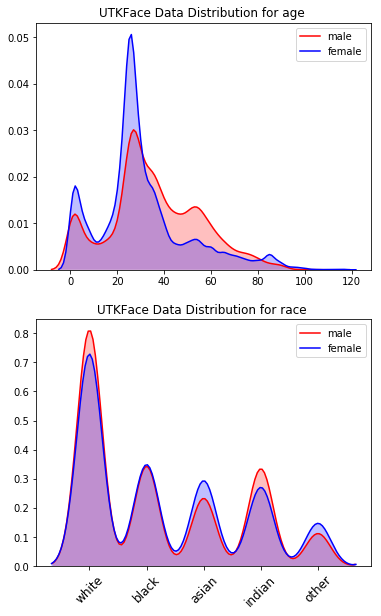
\includegraphics[width=\linewidth]{img/UTKfaces_age-gender-distribution}
\caption{Age and race distribution in the UTKFace data set with respect to the gender.}
\label{fig:fig2}
\end{figure}

The UTKFace data set is available in 2 formats: either "in-the-wild" wherein faces are not explicitly cropped and aligned but contain a single face per image or aligned and cropped to a single face. There are readily available software packages that aid in face detection, image alignment, and cropping and therefore we will not discuss those techniques.\cite{dlib09,mtcnn} To accommodate our compressed time frame and to allow us to explore more interesting aspects of model development and fine-tuning, we will use the cropped and aligned UTKFace data set. Eight randomly chosen images from that data set are shown in Figure \ref{fig:fig1} along with their corresponding age, race, and gender labels at the top of the image. In this subset of images and in general, the labels appear to be correctly assigned for the most part. We did not rigorously evaluate each of the images to verify the labels, but we performed a cursory visual inspection of a few hundred images and found the labels to be correct in more than 95\% of the cases.

\begin{figure*}[ht]\centering % Using \begin{figure*} makes the figure take up the entire width of the page
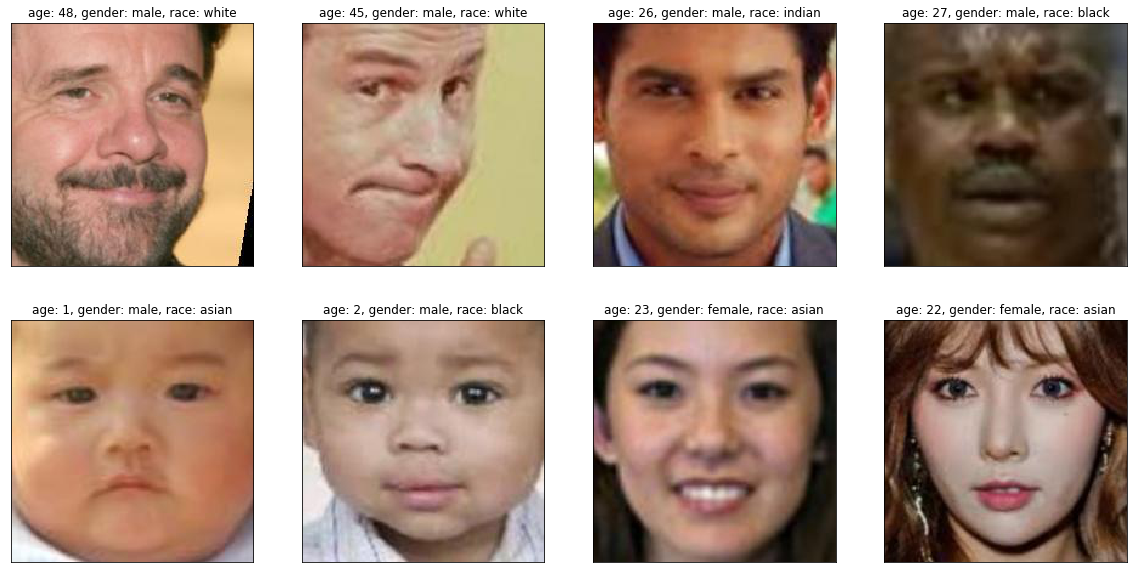
\includegraphics[width=\linewidth]{img/UTKfaces_labelverification}
\caption{A random sampling of images plotted with their labels shows that the UTKFace data set has very accurate labeling.}
\label{fig:fig1}
\end{figure*}

\subsection{Model Selection}
We evaluated several publicly available facial recognition models in the hopes of leveraging them with transfer learning to build our gender classifier. Transfer learning is a nuanced practice, and for our purposes we define it as using pre-trained weights and/or the general architecture of an existing model using similar data to perform a new classification task.\cite{brownlee:transfer,sarkar} A comparison of model complexity in terms of the number of parameters for each model is given in Table \ref{tab:tab2}. 

\begin{table}[hbt]
\caption{Summary of transfer learning models.}
\centering
\begin{tabular}{lclc}
\toprule
%\multicolumn{2}{c}{Name} \\
%\cmidrule(r){1-2}
Model & \# Parameters (million) & Ref \\
\midrule
VGG & 138 & \cite{Simonyan14c} \\
InceptionV3 & 7 & \cite{inceptionv3} \\
ResNet50 & 25.5 & \cite{resnet} \\
\bottomrule
\end{tabular}
\label{tab:tab2}
\end{table}

\noindent Each of the models listed in Table \ref{tab:tab2} are available with pre-trained weights for identity classification. For our purposes, we intend to use a neural network model for the classification of gender in a racially diverse data set. Because none of these models are trained for binary classification of gender, we found that they did not do well in classifying gender out-of-the-box. When the models listed in Table \ref{tab:tab2}, one can either use the full model directly or use only the architecture and trainimag using a different data set. Prior to training, the architecture can be manipulated to perform a new task (e.g., gender classification) or to achieve higher accuracy for different data sets. 

The models listed in Table \ref{tab:tab2} are highly complex with millions of parameters each. We decided to evaluate a much simpler model to juxtapose the possibility that a small architecture tuned with a balanced data set can achieve good accuracy for gender classification. Subedi recently developed a CNN with 674,178 parameters for gender, age, and race classification from the UTKFace data set, and the architecture is shown in Figure \ref{fig:fig3}.s \cite{subedi} Subedi's model architecture consists of 5 2D convolution layers each with a batch normalization layer followed by a 2D maximum pooling layer afterwards. The input layer uses a filter size of 32, and each subsequent convolutional layer multiplies the filter size by an integer corresponding to the layer number (e.g., for concolutional layer 2 the filter size is 32 $\times$ 2). The activation function is a rectified linear unit (ReLU) for all convolutional layers. Subedi uses a so-called 'bottleneck' layer (\mintinline{python}{GlobalMaxPool2D} in Keras) which outputs a 1-dimensional tensor and feeds 3 separate dense layers to produce 3 outputs. In this way, a dense layer is defined for each of the 3 categories each with an appropriate activation function for the type of classification problem (e.g., binary or multiclass). When the model is created, the 3 dense layers are passed in a list as the output. For our purposes, we have adapted the model to output only the gender classification.

\begin{figure*}[ht]\centering % Using \begin{figure*} makes the figure take up the entire width of the page
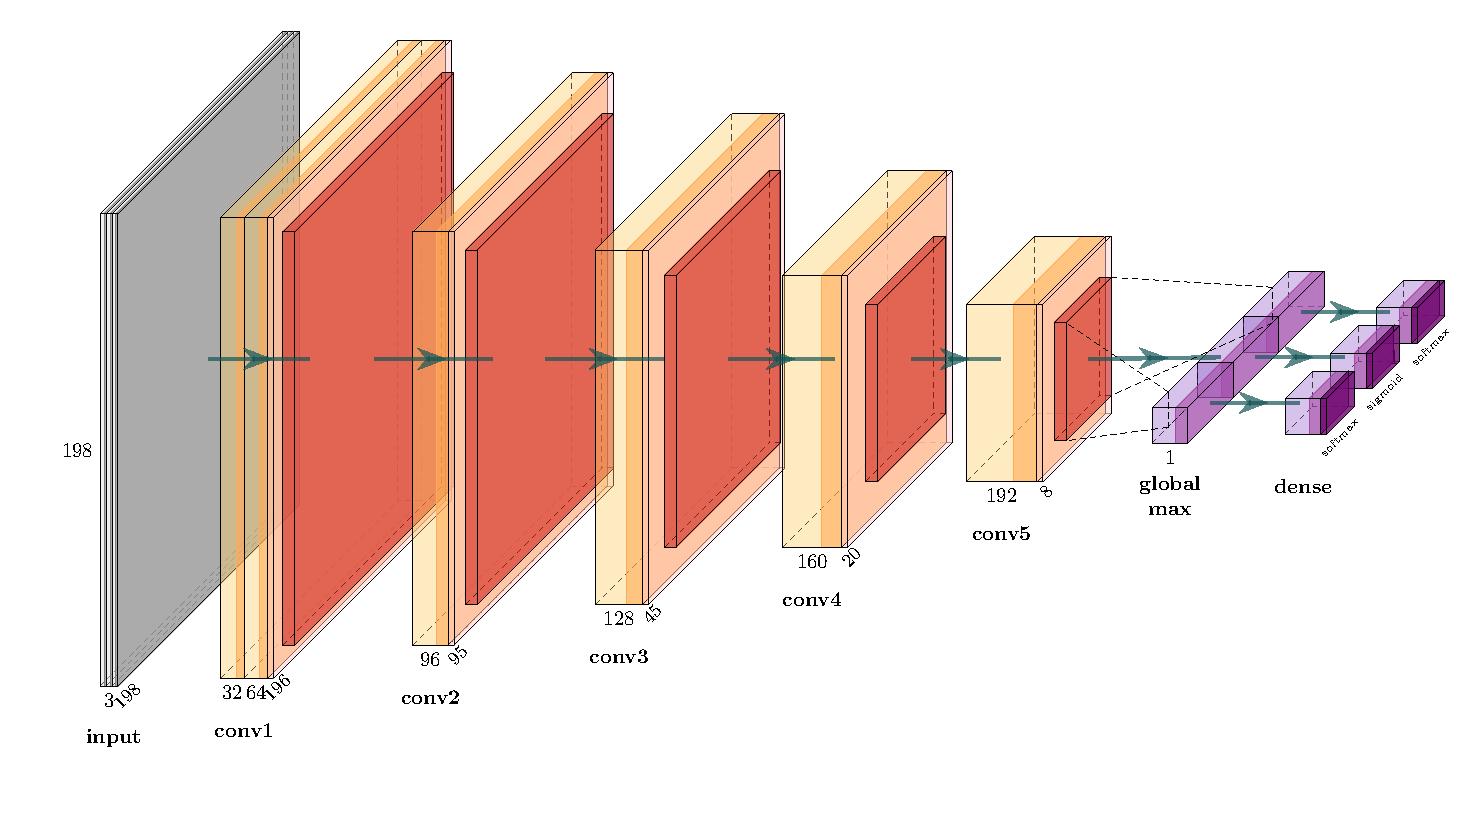
\includegraphics[width=\linewidth]{img/subedi}
\caption{Architecture of neural network developed by Subedi for age, gender, and race classification.}
\label{fig:fig3}
\end{figure*}

\begin{figure*}[hp]\centering % Using \begin{figure*} makes the figure take up the entire width of the page
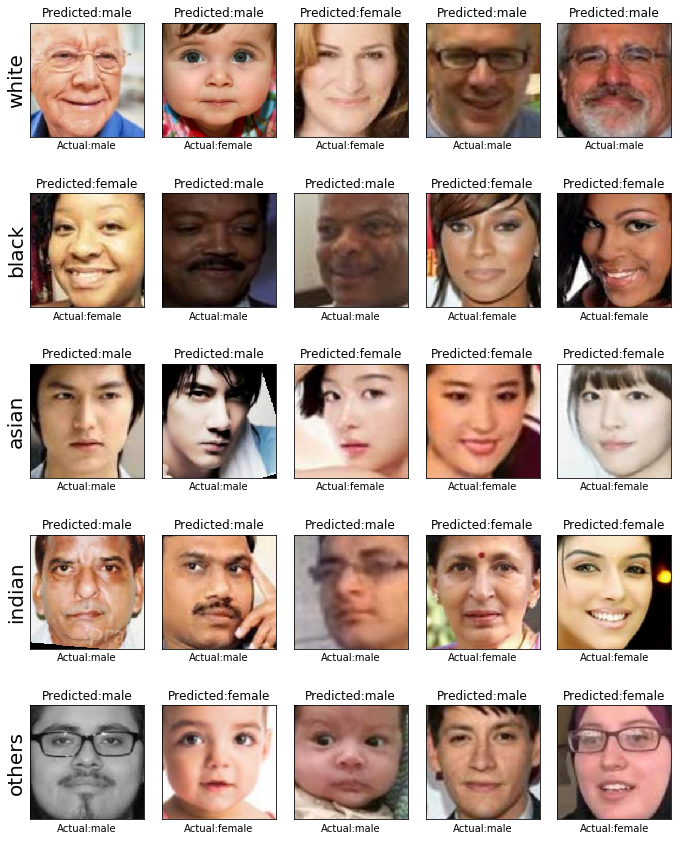
\includegraphics[width=.95\linewidth]{img/base-case-model-results}
\caption{Base case model results with classification results as the top caption and the ground truth as the bottom caption.}
\label{fig:fig4}
\end{figure*}

%------------------------------------------------

\section{Methodology}

Keras with a GPU Tensorflow back end was used for implementing and evaluating CNNs, and all models were run using an NVIDIA Tesla K80 GPU. All code written and used from other sources for this report is given in the accompanying iPython Notebook. 

\subsection{Image Preprocessing}

Data ingestion into the model is not straightforward for large data sets, and can create a bottleneck for feeding the neural network that can cause undesirably high computational times. The goal for any data generator is to leverage all available system resources for ingesting data efficiently so that the bottleneck for computation is not the process of feeding data into the model.\cite{amidi} Keras has a built-in \mintinline{python}{ImageDataGenerator} class, and we evaluated this for some of the models. Generally, though, we found that results were more comprehensible and predictable using our own custom generator based on the one that was developed by Subedi. We found this uniquely useful when applied with UTKFace data because of the relatively small size of the training data set and the CNN. This allowed us to use a simple data generator that takes in image filenames from a data frame and delivers batches of a user-specified size directly to the model through \mintinline{python}{fit_generator}. 

\subsection{Image Augmentation}

One drawback to using a custom data generator is that we could not leverage the convenient functions available in the call to Keras' \mintinline{python}{ImageDataGenerator} for image augementation. As such, we built functionality into our custom generator to add random noise and flip images within the data set as it is ingested into the model. We used the \mintinline{python}{augmenters} class from within the \mintinline{python}{imgaug} package to sequentially augment images by adding black pixels to 2\% of the image (\mintinline{python}{CoarseDropout}) and then flipping the image.  Model was overfitting when flipping only 30\% of the data. When we changed the flip proportion to 50\% then the model performed better. 

We used over-sampling and down-sampling to balance the data set. The 'other' race had the fewest images (1153) in the training data, and we 'down-sampled' the number of images for the other races to include the same number of images. Over-sampling was done by matching the number of images in the race with the most images (white, 6755). Images of races with fewer than 6755 images were added to the training data set by sampling with replacement. The new over-sampled training data set was then passed via the image data generator to the model. Through that pipeline, the image augmentation wrapped inside the data generator ensured that no two images were identical. 

%------------------------------------------------

\section{Results}

Because we began with a broad range of models and data for this work, we began by performing cursory experiments with each model to evaluate 1) computational time, 2) baseline accuracy, and 3) ease of use. Our initial results made it clear that working with the pre-trained models would be computationally prohibitive. We also found that they did not achieve satisfactory results for gender classification. Transfer learning from pre-trained models can be done in three ways: 1) feature extraction, 2) fine tuning, and 3) retraining. 

We evaluated the Resnet50 model both by retraining on the UTKFace cropped data set and by freezing the convolutional base layer and adding a new classification head. We found that gender classification accuracy after training on the UTKFace data set was between 60 - 65\%. In addition to poor accuracy, we found that the training and validation accuracy were between 30 to 40 points off from one another. This indicated that there was a problem with our implementation of our model, but we were not able to troubleshoot it so that we felt comfortable with the results. For the InceptionV3 model, we were able to achieve better gender classification accuracies of more than 90\% but the computational time was long and the complexity of the model made it difficult to interpret results reliably. We attempted to use the VGG16 model, but were unable to get reliable results. Code for these experiments is included with the project documentation. Ultimately, we decided to forgo using one of the pre-trained models and architectures and instead focused on tuning a simple CNN for gender classification. 

\subsection{Base Case Gender Classification}
Using the model developed by Subedi (Figure \ref{fig:fig3}) as a baseline, we adapted the architecture to include a dropout layers between the convolutional and batch normalization layers. The dropout layers are a form of regularizer that randomly drop neurons from the network. In doing this, other neurons in the network must do the work of the dropped neuron thereby making it less probable that a single neuron performs a single task in the model. As a result, as the network learns from the training data set it becomes more capable of generalizing to randomness thereby reducing the probability of overfitting.

The base case training for the gender classified was done using a batch size of 64, a base filter size of 16, and 10 epochs. The softmax activation function was used to do the binary classification and the categorical crossentropy loss function was used to calculate loss. We used the RMSProp optimizer because it yielded superior results. Results from the base case model are shown in Figure \ref{fig:fig4} for each of the race categories that we studied. In this small subset of images chosen at random from the validation data set, there is only one incorrect gender assignment. During training, the training accuracy reached just under 92\% whereas the validation accuracy hovered around 90\%. These are excellent baseline error rates, and the simple model architecture appears to perform very well even with only very cursory development. 

\subsection{Effect of Data Set Balancing}

One of the main issues to which algorithmic bias has been attributed is the issue of racial imbalance in training data sets. To overcome this, we evaluated the effect of using over-sampling and down-sampling to eliminate algorithmic bias. A comparison of model performance for f1 score by gender and race is given in Table \ref{tab:tab3}.

\begin{table}[hbt]
\caption{F1 scores for all 3 models by race.}
\centering
\begin{tabular}{lcccccc}
\toprule
& \multicolumn{2}{c}{Baseline} & \multicolumn{2}{c}{Down-Sampling} & \multicolumn{2}{c}{Over-Sampling}\\
\cmidrule(r){1-7}
 & M & F & M & F & M & F \\
\midrule
White & 0.91 & 0.9 & 0.88 & 0.86 & 0.95 & 0.94\\
Black & 0.93 & 0.93 & 0.9 & 0.89 & 0.93 & 0.92\\
Asian & 0.92 & 0.95 & 0.87 & 0.91 & 0.93 & 0.95 \\
Indian & 0.92 & 0.88 & 0.89 & 0.84 & 0.95 & 0.92 \\
Other & 0.91 & 0.93 & 0.88 & 0.90 & 0.93 & 0.94 \\
\bottomrule
\multicolumn{7}{l}{M = male, F = female}
\end{tabular}
\label{tab:tab3}
\end{table}

Down-sampling the data for each race to the same number of images for the least represented race (other) reduced the training data set by over 70\%. The reduction in the size of the training data set did not strongly inhibit the training accuracy which remained close to 90\%. The validation accuracy was nearly 5 points worse than the baseline model with an average validation accuracy of around 85\%. The overall misclassification rate for the down-sample trained model was over 13\%. This is slightly higher than the baseline model misclassification rate of 12.4\%. The down-sampled model did have better precision (85.3\%) than the baseline model (82.4\%) indicating that though the overall accuracy was lower it predicted more true positives per predicted true value. The down-sampling model computational time was similar to that of the baseline model, and 10 epochs were completed in a little over 10 minutes. Overall, though, the down-sampled model was not a significant improvement over the baseline model.

\begin{figure}[ht]\centering % Using \begin{figure*} makes the figure take up the entire width of the page
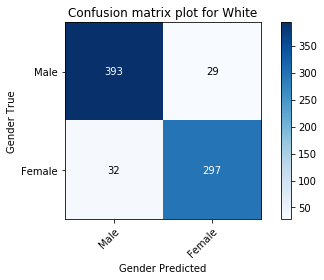
\includegraphics[width=.95\linewidth]{img/confmat_white}
\caption{Confusion matrix for race = white from the optimal gender classification model.}
\label{fig:fig5}
\end{figure}

Over-sampling, the practice of adding redundant images to the data set by random sampling and replacement, facilitated an improvement in overall modeling accuracy. To visualize the model performance by race, we plotted the confusion matrices for each race individually as shown in Figure \ref{fig:fig:5} (white) and Figure \ref{fig:fig:6} (black). All confusion matrix plots are given in the accompanying notebook, but a table summarizing the precision and misclassification rates by race is given in Table \ref{tab:tab4}. 

\begin{table}[hbt]
\caption{Overall precision and misclassification rates for the tuned model by race.}
\centering
\begin{tabular}{lccc}
\toprule
%\multicolumn{2}{c}{Name} \\
%\cmidrule(r){1-2}
Race & Precision & Misclassification Rate \\
\midrule
White & 91\% & 8\% \\
Black & 92\% & 12\% \\
Asian & 94\% & 6\% \\
Indian & 94\% & 6\% \\
Other & 94\% & 6\% \\
\bottomrule
\end{tabular}
\label{tab:tab4}
\end{table}

\noindent In the baseline model, the average gender classification precision was 88\% for black and white, 94\% for indian, 93\% for asian, and 91\% for other. Though our model does not offer a huge improvement and totally equity, we have produced a model that has higher precision for 4 of the 5 races. Furthermore, the model has a higher overall accuracy for gender prediction and better than 90\% precision for all races. We surmise based on these results that over-sampling and adding back augmented images improves the models ability to classify gender and reduces model bias.

\begin{figure}[ht]\centering % Using \begin{figure*} makes the figure take up the entire width of the page
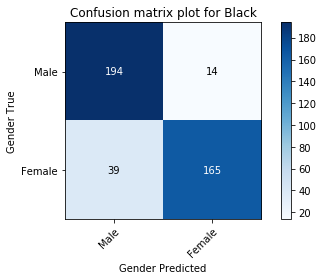
\includegraphics[width=.95\linewidth]{img/confmat_black}
\caption{Confusion matrix for race = black from the optimal gender classification model.}
\label{fig:fig6}
\end{figure}

%\begin{figure}[ht]\centering % Using \begin{figure*} makes the figure take up the entire width of the page
%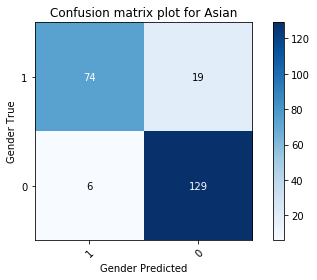
\includegraphics[width=.95\linewidth]{img/confmat_asian}%
%\caption{Confusion matrix for race = asian from the optimal gender classification model.}
%\label{fig:fig9}
%\end{figure}

\subsection{Feature Representation Mapping}

\begin{figure*}[ht]\centering % Using \begin{figure*} makes the figure take up the entire width of the page
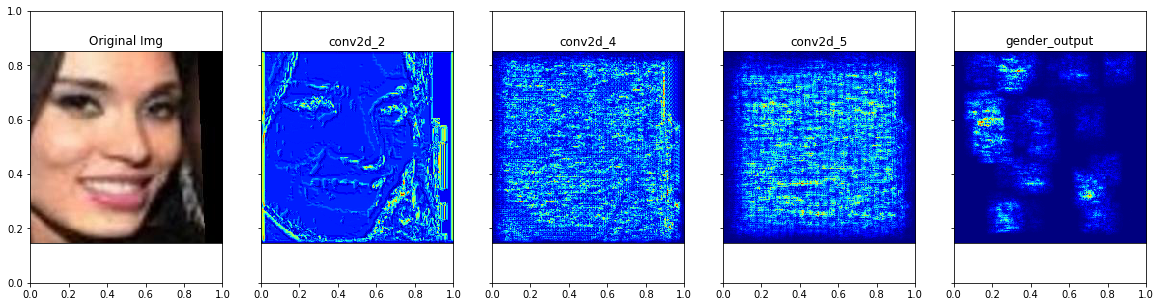
\includegraphics[width=.95\linewidth]{img/saliency}
\caption{Saliency map for consecutive convolutional layers demonstrating the progression from a raw image to only the most important facial features.}
\label{fig:fig7}
\end{figure*}

It is informative to visualize the important features in an image that contributes to its classification in a neural network. For our tuned model, we used saliency maps to elucidate the important facial features from different races that contribute to their classification as males or females. A series of saliency maps from convolutional layers throughout the model is shown in Figure \ref{fig:fig7} and demonstrates the progression from a full face image to only the most pertinent features. As the model progresses through the layers, the edges in the face are isolated then reduced to a handful of regions in the face that are unique. Ultimately, the features in the face left are the forehead, cheek bones, nose, mouth, eyes, and chin area. 


Evaluating saliency mapping and its relationship with feature distinctions between races is beyond the scope of this project, but we considered the idea of uses PCA to elucidated important features and evaluating bias in a classified built from that analysis. There are examples in the literature for performing PCA on the landmark features data for images, and extracting Eigenvectors which can then be used for created support vector machines (SVM). This would be an interesting way to build a gender classifier, and the idea of producing a neural net-free classifier poses prospects for much faster models. 

\subsection{Validation with Other Data Sets}
We revisited the original facial image data set (VGGFace2) that we began the project with to validate our gender classification model. We tested a total of 30 images with 6 images from each race. We used a very small sample size because we had to manually label both the gender and the race. Though this is not a comprehensive evaluation of the model, it serves as a useful check to see if the model is useful for other data sets with different image quality. Prior to evaluating the images, they were preprocessed using the \mintinline{python}{dlib} package. This allowed us to use the complex 'in-the-wild' images directly. Using the 68 face landmark shape detector from \mintinline{python}{dlib}, we were able to detect and isolate only the faces in each image.

The cropped images from the VGGFace2 data set were saved and used as a validation data set with the over-sampled model. A comparison of raw images from the VGGface2 with corresponding predicted gender and ground truth labels are shown in Figure \ref{fig:fig8}. The model achieved a precision of 100\%, but had a misclassification rate of 40\%. The low sample size probably contributed greatly to these results, but we built and demonstrated a gender classifier from a fairly simple CNN architecture that is extensible to dissimilar data sets. Our research into pre-trained models indicated that this is relatively uncommon and that benchmarks are so tightly bounded that it is difficult for even the most precise and highest accuracy models to achieve adequate classification on other data sets. Because of this, we put forth that the model we have developed not only reduced racial bias but is also sufficient for use with data sets other than the one that it was trained with.

\begin{figure*}[ht]\centering % Using \begin{figure*} makes the figure take up the entire width of the page
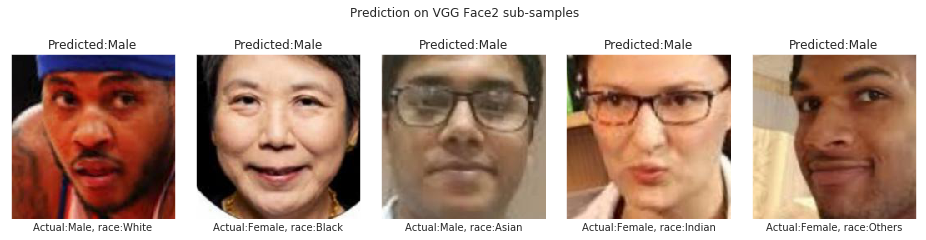
\includegraphics[width=.95\linewidth]{img/VGG_facelabels}
\caption{Confusion matrix for race = white from the optimal gender classification model.}
\label{fig:fig8}
\end{figure*}

\section{Conclusions}
During this project, we improved a classifier for gender prediction from racially heterogeneous images using a relatively simple CNN. Recently, there has been media coverage of so-called 'algorithmic bias' that is the result of imbalanced training data sets. As a result, widespread algorithmic bias has crept into popular, publicly available pre-trained models such as Google's Inception, Microsoft's ResNet, and the VGG group's VGG models. Our approach to investigating this issue was twofold: we evaluated whether pre-trained models were necessary for producing an accurate gender classifier and we developed and tuned a CNN for gender classification. Pre-trained models are incredibly valuable, and will continue to provide the groundwork for building complex, diverse, and extensible models. However, in our work we found that because the aforementioned pre-trained models are not meant specifically for gender classification, they cannot be used out of the box for such a task. We applied methods for adapting these models to gender classification including training the unchanged architecture with racially balanced data sets for gender classification and freezing certain layers and retraining the convolutional head layer (feature extraction). We found the models to be difficult to work with and computationally expensive which lead us to the question of whether we could reduce algorithmic racial bias using a simpler model.

We leveraged an existing CNN architecture for gender classification and fine-tuned it to produce higher accuracy and less algorithmic bias. We achieved this by implementing image augmentation in the form of down-sampling and over-sampling. When over-sampling, we randomly selected images to add back to the training data set, but flipped and added noise to the resampled images. The main conclusions from this work were:

\begin{itemize}
\item Pre-trained models can be useful in certain circumstances, but are difficult to work with, computationally expensive, and might not fit the needs for the particular classifier that is desired
\item Algorithmic bias can be reduced when balancing the training data set by race 
\item Down-sampling, removing images to balance the training data set, results in lower modeling accuracy because of the reduced training data set size
\item Over-sampling, adding images by resampling with noise/translation, improves modeling accuracy 
\end{itemize}
%------------------------------------------------

\phantomsection
\phantomsection
\phantomsection
\phantomsection
\phantomsection
\phantomsection

%----------------------------------------------------------------------------------------
%	REFERENCE LIST
%----------------------------------------------------------------------------------------
\phantomsection
\Urlmuskip=0mu plus 2mu\relax
\bibliographystyle{unsrt}
\bibliography{references}

%----------------------------------------------------------------------------------------

\end{document}